\section{问题一：典型日确定性储能调度}
\subsection{线性规划模型}
对给定的典型日，决策变量为购电$x_t$、充电$c_t$、放电$q_t$、电量$E_t$及弃光$s_t$。
在不需要紧急购电的确定性条件下，目标为
\begin{equation}\min C_1=\sum_{t=1}^{T}p_tx_t.\label{eq:q1obj}\end{equation}
每个槽满足供需平衡与储能递推：
\begin{align}
P_t+x_t+q_t&=L_t+c_t+s_t,\label{eq:balance}\\
E_t&=E_{t-1}+\eta c_t-q_t/\eta.\label{eq:soc}
\end{align}
充电量从电网侧计量，故进入电池的电量为$\eta c_t$；向负荷放出$q_t$需消耗$q_t/\eta$。
容量、功率、非负性与循环条件为
\begin{align}
1200\leq E_t\leq10800,\quad &0\leq c_t,q_t\leq5000/6,\label{eq:bounds}\\
x_t\geq0,\quad 0\leq s_t\leq P_t,\quad &E_0=E_T=6000.\label{eq:cycle}
\end{align}
所有约束与目标均为线性，共720个变量、289条等式约束，采用稀疏矩阵和HiGHS求解。
线性规划算法可高效求解该规模问题\cite{huangfu2018}。模型未引入充放互斥二元变量，因此解后必须检查同槽同时充放；所得正式解通过该项检查。
\subsection{最优策略与题目指定结果}
最优全天购电量为59482.7 kWh，购电费为35126.95元，较无储能基线节省26.9\%。
电池利用低价时段充电，在高价及光伏不足时段释放电能，全天弃光为0。
题面指定的购电及储能结果列于表\ref{tab:q1buy}、表\ref{tab:q1soc}。
\begin{table}[htbp]\centering
\caption{问题一指定时段购电量（kWh）}\label{tab:q1buy}
\small
\begin{tabular}{cr}
\toprule
时间段 & 购电量 \\
\midrule
10:00-10:10 & 0.00 \\
12:00-12:10 & 486.40 \\
14:00-14:10 & 0.00 \\
16:00-16:10 & 394.93 \\
18:00-18:10 & 636.98 \\
20:00-20:10 & 0.00 \\
\midrule 全天购电量 & 59482.7 \\
全天购电费/元 & 35126.95 \\
\bottomrule
\end{tabular}
\end{table}
\begin{table}[htbp]\centering
\caption{问题一指定区间储能充放电量（kWh）}\label{tab:q1soc}
\small
\begin{tabular}{crr}
\toprule
时间段 & 充电量 & 放电量 \\
\midrule
0:00-4:00 & 4500.00 & 0.00 \\
4:00-8:00 & 833.33 & 6365.84 \\
8:00-12:00 & 4787.96 & 1703.00 \\
12:00-16:00 & 5286.04 & 91.10 \\
16:00-20:00 & 0.00 & 5780.13 \\
20:00-24:00 & 5333.33 & 2859.87 \\
\midrule 0:00储电量 & \multicolumn{2}{c}{6000.00} \\
24:00储电量 & \multicolumn{2}{c}{6000.00} \\
\bottomrule
\end{tabular}
\end{table}

\begin{figure}[htbp]\centering
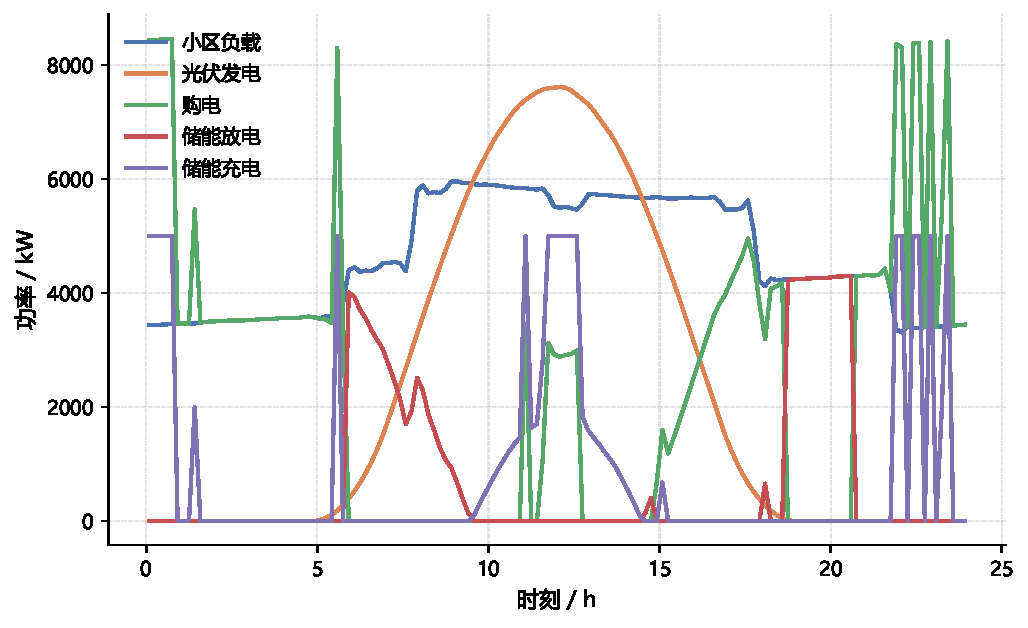
\includegraphics[width=.92\textwidth]{../../figures/Q1_调度时序.pdf}
\caption{典型日购电、光伏与储能联合调度}\label{fig:q1}
\end{figure}
图\ref{fig:q1}中的充放电时序同时受峰谷价格和光伏出力影响。由于循环条件约束日末电量，全天节省不是通过消耗初始储能获得的暂时收益。
四小时汇总区间内可能同时出现正的累计充电与放电量，这表示不同10分钟槽采用不同动作，不意味着同槽同时充放。
\questionconclusion{确定性典型日最优购电费为35126.95元，储能节省比例26.9\%；该模型提供后续各问共用的物理约束。}
